% Decoder with skips
% Made with Xematics. Positions are in px (1 px = 0.75 pt), as in the SVG export.
\documentclass[tikz, border=4pt]{standalone}
\definecolor{xm1}{HTML}{FFFFFF}
\definecolor{xm2}{HTML}{D4E8F5}
\definecolor{xm3}{HTML}{0072B2}
\definecolor{xm4}{HTML}{F1F2F4}
\definecolor{xm5}{HTML}{4B5563}
\definecolor{xm6}{HTML}{DFE3E8}
\definecolor{xm7}{HTML}{FBE8C4}
\definecolor{xm8}{HTML}{B97800}
\definecolor{xm9}{HTML}{AEB3B9}
\definecolor{xm10}{HTML}{6B7280}
\definecolor{xm11}{HTML}{1F2937}
\begin{document}
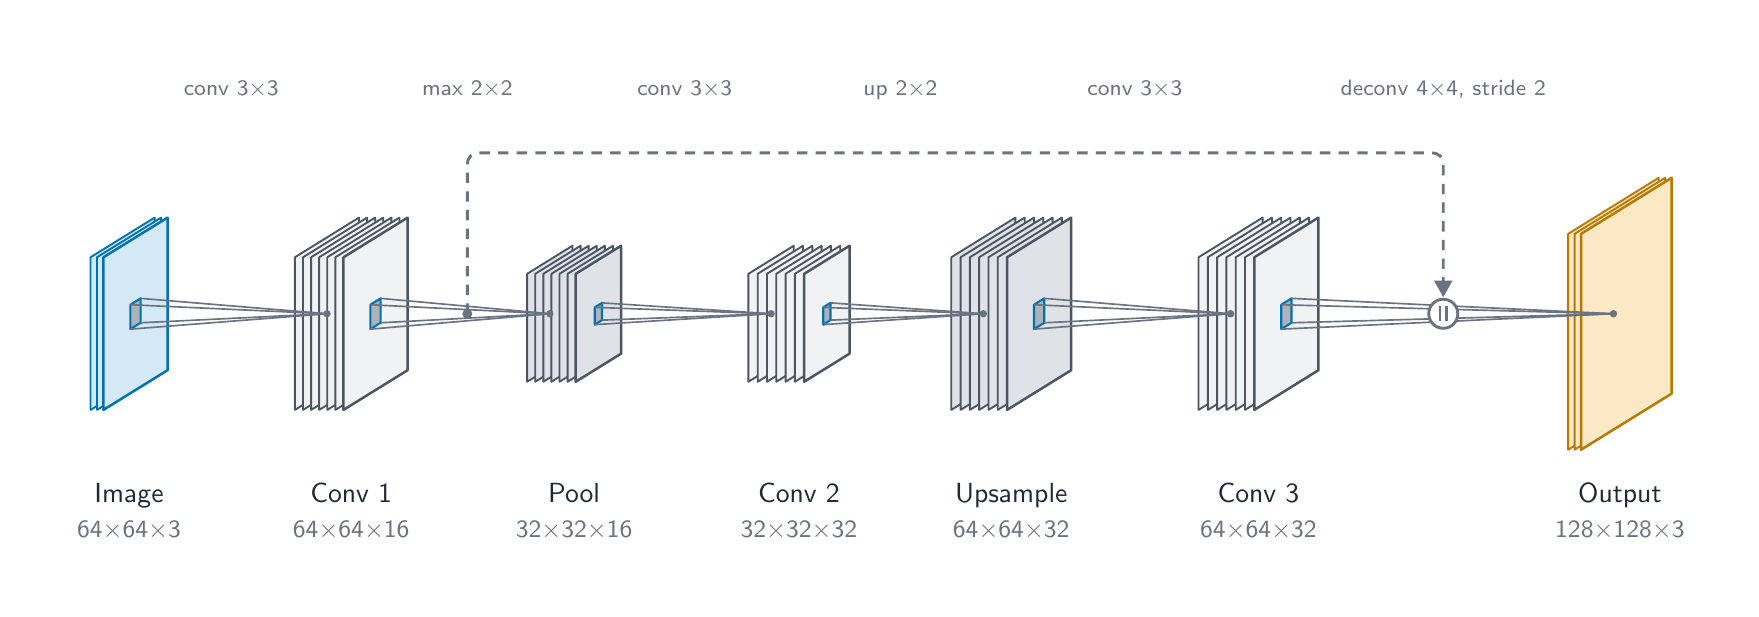
\begin{tikzpicture}[x=0.75pt, y=-0.75pt]
  \tikzset{
    xm map input back/.style={fill=xm2, draw=xm3, line width=0.68pt, line join=round},
    xm map input/.style={fill=xm2, draw=xm3, line width=0.9pt, line join=round},
    xm map hidden back/.style={fill=xm4, draw=xm5, line width=0.68pt, line join=round},
    xm map hidden/.style={fill=xm4, draw=xm5, line width=0.9pt, line join=round},
    xm map pool back/.style={fill=xm6, draw=xm5, line width=0.68pt, line join=round},
    xm map pool/.style={fill=xm6, draw=xm5, line width=0.9pt, line join=round},
    xm map output back/.style={fill=xm7, draw=xm8, line width=0.68pt, line join=round},
    xm map output/.style={fill=xm7, draw=xm8, line width=0.9pt, line join=round},
    xm window/.style={fill=xm9, draw=xm3, line width=0.75pt, line join=round},
    xm ray/.style={draw=xm10, line width=0.6pt},
    xm ray end/.style={fill=xm10},
    xm skip start/.style={fill=xm10},
    xm skip concat/.style={fill=none, draw=xm10, line width=1.05pt, dash pattern=on 3.75pt off 3pt, line join=round},
    xm skip head/.style={fill=xm10},
    xm join/.style={fill=xm1, draw=xm10, line width=1.05pt},
    xm join sign/.style={fill=none, draw=xm10, line width=1.05pt},
    xm name xm11/.style={text=xm11, inner sep=0, font=\sffamily\fontsize{9.75}{11.7}\selectfont},
    xm size xm10/.style={text=xm10, inner sep=0, font=\sffamily\fontsize{9}{10.8}\selectfont},
    xm op xm10/.style={text=xm10, inner sep=0, font=\sffamily\fontsize{8.25}{9.9}\selectfont},
  }
  \fill[xm1] (0,0) rectangle (820.39,270.6);
  % Layers
  \draw[xm map input back] (30.29,110.62) -- (61.18,91.5) -- (61.18,165.04) -- (30.29,184.16) -- cycle;
  \draw[xm map input back] (33.4,110.62) -- (64.28,91.5) -- (64.28,165.04) -- (33.4,184.16) -- cycle;
  \draw[xm map input] (36.5,110.62) -- (67.39,91.5) -- (67.39,165.04) -- (36.5,184.16) -- cycle;
  \draw[xm map hidden back] (128.75,110.62) -- (159.64,91.5) -- (159.64,165.04) -- (128.75,184.16) -- cycle;
  \draw[xm map hidden back] (132.65,110.62) -- (163.54,91.5) -- (163.54,165.04) -- (132.65,184.16) -- cycle;
  \draw[xm map hidden back] (136.55,110.62) -- (167.44,91.5) -- (167.44,165.04) -- (136.55,184.16) -- cycle;
  \draw[xm map hidden back] (140.45,110.62) -- (171.34,91.5) -- (171.34,165.04) -- (140.45,184.16) -- cycle;
  \draw[xm map hidden back] (144.35,110.62) -- (175.24,91.5) -- (175.24,165.04) -- (144.35,184.16) -- cycle;
  \draw[xm map hidden back] (148.25,110.62) -- (179.14,91.5) -- (179.14,165.04) -- (148.25,184.16) -- cycle;
  \draw[xm map hidden] (152.15,110.62) -- (183.04,91.5) -- (183.04,165.04) -- (152.15,184.16) -- cycle;
  \draw[xm map pool back] (240.64,118.59) -- (262.48,105.07) -- (262.48,157.07) -- (240.64,170.59) -- cycle;
  \draw[xm map pool back] (244.54,118.59) -- (266.38,105.07) -- (266.38,157.07) -- (244.54,170.59) -- cycle;
  \draw[xm map pool back] (248.44,118.59) -- (270.28,105.07) -- (270.28,157.07) -- (248.44,170.59) -- cycle;
  \draw[xm map pool back] (252.34,118.59) -- (274.18,105.07) -- (274.18,157.07) -- (252.34,170.59) -- cycle;
  \draw[xm map pool back] (256.24,118.59) -- (278.08,105.07) -- (278.08,157.07) -- (256.24,170.59) -- cycle;
  \draw[xm map pool back] (260.14,118.59) -- (281.98,105.07) -- (281.98,157.07) -- (260.14,170.59) -- cycle;
  \draw[xm map pool] (264.04,118.59) -- (285.88,105.07) -- (285.88,157.07) -- (264.04,170.59) -- cycle;
  \draw[xm map hidden back] (347.24,118.59) -- (369.08,105.07) -- (369.08,157.07) -- (347.24,170.59) -- cycle;
  \draw[xm map hidden back] (351.72,118.59) -- (373.56,105.07) -- (373.56,157.07) -- (351.72,170.59) -- cycle;
  \draw[xm map hidden back] (356.2,118.59) -- (378.04,105.07) -- (378.04,157.07) -- (356.2,170.59) -- cycle;
  \draw[xm map hidden back] (360.68,118.59) -- (382.52,105.07) -- (382.52,157.07) -- (360.68,170.59) -- cycle;
  \draw[xm map hidden back] (365.16,118.59) -- (387,105.07) -- (387,157.07) -- (365.16,170.59) -- cycle;
  \draw[xm map hidden back] (369.64,118.59) -- (391.48,105.07) -- (391.48,157.07) -- (369.64,170.59) -- cycle;
  \draw[xm map hidden] (374.12,118.59) -- (395.96,105.07) -- (395.96,157.07) -- (374.12,170.59) -- cycle;
  \draw[xm map pool back] (444.99,110.62) -- (475.88,91.5) -- (475.88,165.04) -- (444.99,184.16) -- cycle;
  \draw[xm map pool back] (449.47,110.62) -- (480.36,91.5) -- (480.36,165.04) -- (449.47,184.16) -- cycle;
  \draw[xm map pool back] (453.95,110.62) -- (484.84,91.5) -- (484.84,165.04) -- (453.95,184.16) -- cycle;
  \draw[xm map pool back] (458.43,110.62) -- (489.32,91.5) -- (489.32,165.04) -- (458.43,184.16) -- cycle;
  \draw[xm map pool back] (462.91,110.62) -- (493.8,91.5) -- (493.8,165.04) -- (462.91,184.16) -- cycle;
  \draw[xm map pool back] (467.39,110.62) -- (498.28,91.5) -- (498.28,165.04) -- (467.39,184.16) -- cycle;
  \draw[xm map pool] (471.87,110.62) -- (502.75,91.5) -- (502.75,165.04) -- (471.87,184.16) -- cycle;
  \draw[xm map hidden back] (564.12,110.62) -- (595,91.5) -- (595,165.04) -- (564.12,184.16) -- cycle;
  \draw[xm map hidden back] (568.6,110.62) -- (599.48,91.5) -- (599.48,165.04) -- (568.6,184.16) -- cycle;
  \draw[xm map hidden back] (573.08,110.62) -- (603.96,91.5) -- (603.96,165.04) -- (573.08,184.16) -- cycle;
  \draw[xm map hidden back] (577.55,110.62) -- (608.44,91.5) -- (608.44,165.04) -- (577.55,184.16) -- cycle;
  \draw[xm map hidden back] (582.03,110.62) -- (612.92,91.5) -- (612.92,165.04) -- (582.03,184.16) -- cycle;
  \draw[xm map hidden back] (586.51,110.62) -- (617.4,91.5) -- (617.4,165.04) -- (586.51,184.16) -- cycle;
  \draw[xm map hidden] (590.99,110.62) -- (621.88,91.5) -- (621.88,165.04) -- (590.99,184.16) -- cycle;
  \draw[xm map output back] (742.17,99.35) -- (785.85,72.31) -- (785.85,176.31) -- (742.17,203.35) -- cycle;
  \draw[xm map output back] (745.28,99.35) -- (788.96,72.31) -- (788.96,176.31) -- (745.28,203.35) -- cycle;
  \draw[xm map output] (748.39,99.35) -- (792.07,72.31) -- (792.07,176.31) -- (748.39,203.35) -- cycle;
  \draw[xm window] (49.47,133.48) -- (54.42,130.42) -- (54.42,142.18) -- (49.47,145.24) -- cycle;
  \draw[xm ray] (49.47,133.48) -- (144.19,137.83);
  \draw[xm ray] (54.42,130.42) -- (144.19,137.83);
  \draw[xm ray] (54.42,142.18) -- (144.19,137.83);
  \draw[xm ray] (49.47,145.24) -- (144.19,137.83);
  \fill[xm ray end] (144.19,137.83) circle[radius=1.8];
  \draw[xm window] (165.12,133.48) -- (170.06,130.42) -- (170.06,142.18) -- (165.12,145.24) -- cycle;
  \draw[xm ray] (165.12,133.48) -- (251.56,137.83);
  \draw[xm ray] (170.06,130.42) -- (251.56,137.83);
  \draw[xm ray] (170.06,142.18) -- (251.56,137.83);
  \draw[xm ray] (165.12,145.24) -- (251.56,137.83);
  \fill[xm ray end] (251.56,137.83) circle[radius=1.8];
  \draw[xm window] (273.21,134.75) -- (276.71,132.59) -- (276.71,140.91) -- (273.21,143.07) -- cycle;
  \draw[xm ray] (273.21,134.75) -- (358.16,137.83);
  \draw[xm ray] (276.71,132.59) -- (358.16,137.83);
  \draw[xm ray] (276.71,140.91) -- (358.16,137.83);
  \draw[xm ray] (273.21,143.07) -- (358.16,137.83);
  \fill[xm ray end] (358.16,137.83) circle[radius=1.8];
  \draw[xm window] (383.29,134.75) -- (386.79,132.59) -- (386.79,140.91) -- (383.29,143.07) -- cycle;
  \draw[xm ray] (383.29,134.75) -- (460.43,137.83);
  \draw[xm ray] (386.79,132.59) -- (460.43,137.83);
  \draw[xm ray] (386.79,140.91) -- (460.43,137.83);
  \draw[xm ray] (383.29,143.07) -- (460.43,137.83);
  \fill[xm ray end] (460.43,137.83) circle[radius=1.8];
  \draw[xm window] (484.84,133.48) -- (489.78,130.42) -- (489.78,142.18) -- (484.84,145.24) -- cycle;
  \draw[xm ray] (484.84,133.48) -- (579.56,137.83);
  \draw[xm ray] (489.78,130.42) -- (579.56,137.83);
  \draw[xm ray] (489.78,142.18) -- (579.56,137.83);
  \draw[xm ray] (484.84,145.24) -- (579.56,137.83);
  \fill[xm ray end] (579.56,137.83) circle[radius=1.8];
  \draw[xm window] (603.97,133.48) -- (608.91,130.42) -- (608.91,142.18) -- (603.97,145.24) -- cycle;
  \draw[xm ray] (603.97,133.48) -- (764.01,137.83);
  \draw[xm ray] (608.91,130.42) -- (764.01,137.83);
  \draw[xm ray] (608.91,142.18) -- (764.01,137.83);
  \draw[xm ray] (603.97,145.24) -- (764.01,137.83);
  \fill[xm ray end] (764.01,137.83) circle[radius=1.8];
  % Skip connections
  \path[xm skip start] (211.84,137.83) circle[radius=2.4];
  \draw[xm skip concat] (211.84,137.83) -- (211.84,66.31) .. controls (211.84,62.31) and (213.84,60.31) .. (217.84,60.31) -- (676.03,60.31) .. controls (680.03,60.31) and (682.03,62.31) .. (682.03,66.31) -- (682.03,123.83);
  \fill[xm skip head] (682.03,129.83) -- (677.53,121.83) -- (686.53,121.83) -- cycle;
  \path[xm join] (682.03,137.83) circle[radius=7];
  \draw[xm join sign] (680.43,134.33) -- (680.43,141.33) (683.63,134.33) -- (683.63,141.33);
  % Labels
  \node[xm name xm11, anchor=base] at (48.84,228.94) {Image};
  \node[xm size xm10, anchor=base] at (48.84,245.7) {64\ensuremath{\times}64\ensuremath{\times}3};
  \node[xm op xm10, anchor=base] at (98.07,32.66) {conv 3\ensuremath{\times}3};
  \node[xm name xm11, anchor=base] at (155.89,228.94) {Conv 1};
  \node[xm size xm10, anchor=base] at (155.89,245.7) {64\ensuremath{\times}64\ensuremath{\times}16};
  \node[xm op xm10, anchor=base] at (211.84,32.66) {max 2\ensuremath{\times}2};
  \node[xm name xm11, anchor=base] at (263.26,228.94) {Pool};
  \node[xm size xm10, anchor=base] at (263.26,245.7) {32\ensuremath{\times}32\ensuremath{\times}16};
  \node[xm op xm10, anchor=base] at (316.56,32.66) {conv 3\ensuremath{\times}3};
  \node[xm name xm11, anchor=base] at (371.6,228.94) {Conv 2};
  \node[xm size xm10, anchor=base] at (371.6,245.7) {32\ensuremath{\times}32\ensuremath{\times}32};
  \node[xm op xm10, anchor=base] at (420.47,32.66) {up 2\ensuremath{\times}2};
  \node[xm name xm11, anchor=base] at (473.87,228.94) {Upsample};
  \node[xm size xm10, anchor=base] at (473.87,245.7) {64\ensuremath{\times}64\ensuremath{\times}32};
  \node[xm op xm10, anchor=base] at (533.44,32.66) {conv 3\ensuremath{\times}3};
  \node[xm name xm11, anchor=base] at (593,228.94) {Conv 3};
  \node[xm size xm10, anchor=base] at (593,245.7) {64\ensuremath{\times}64\ensuremath{\times}32};
  \node[xm op xm10, anchor=base] at (682.03,32.66) {deconv 4\ensuremath{\times}4, stride 2};
  \node[xm name xm11, anchor=base] at (767.12,228.94) {Output};
  \node[xm size xm10, anchor=base] at (767.12,245.7) {128\ensuremath{\times}128\ensuremath{\times}3};
\end{tikzpicture}
\end{document}
